\section{Selecci�n de las arquitecturas}

\begin{frame}
    \begin{center}
	\Huge SELECCI�N DE LAS ARQUITECTURAS
	\end{center}
\end{frame}

\subsection{Transformada de Fourier}

\begin{frame}{Algoritmos FFT}
  %\begin{block}{Comparativa de los algoritmos FFT}
%   \begin{itemize}
%     \item<1-> Comparativa de los algoritmos FFT
% 	\begin{center}
% 	  \advance\leftskip-0.2cm
% 	  {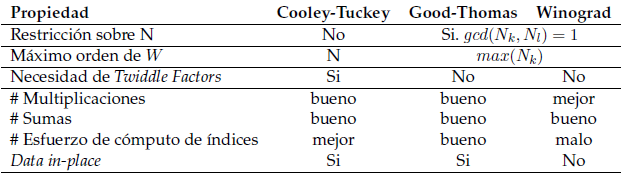
\includegraphics[scale=0.45]{./figures/FFT_table.png}}
%     \end{center}
%   %\end{block}
%   
%   \item<2-> Selección
%     \begin{itemize}
%       \item<2-> Se decide implementar una arquitectura basada en el algoritmo
%       Cooley-Tuckey.
%       \item<3-> Se implementará la versión del algoritmo en que los sub-cómputos son del mismo
%       tamaño, conocidos como radix-r.
%     \end{itemize}
%   \end{itemize}
  \begin{itemize}
    \Fontit
    \item<1-> Existen varios algoritmos
    \begin{itemize}
      \Fontitit
      \item<2-> Good-Thomas
      \item<3-> Winograd
      \item<4-> Cooley-Tuckey
    \end{itemize} 
    \item<5-> Se selecciona el algoritmo Radix-r (Cooley-Tuckey)
    \begin{itemize}
      \Fontitit
      \item<6-> Flexibilidad en la longitud
      \item<7-> Simplicidad en la implementaci�n
      \item<8-> Posibilidad de reutilizar m�dulos
    \end{itemize}
  \end{itemize}
\end{frame}

\begin{frame}{Cantidad de puntos por operaci�n}
  \begin{itemize}
%     \item<1-> A mayor longitud de las DFTs interiores es menor la cantidad de DFTs interiores a
%     realizar. Pero aumentan la cantidad de operaciones por DFT.
    \item<1-> Cantidad de etapas
    \item<2-> Cantidad de operaciones por etapa
    \vfill
    
    \uncover<3->{\begin{tabular}{c c c c}
		\textbf{Long. del bloque} & \textbf{Mult.} & \textbf{Mult. no triv} &
		\textbf{sumas} \\ \hline 
		$2$ & $2$ & \color<3->[rgb]{1,0,0}$0$ & $2$ \\
		$3$ & $3$ & $2$ & $6$ \\
		$4$ & $4$ & \color<3->[rgb]{1,0,0}$0$ & $8$ \\
		$5$ & $6$ & $5$ & $17$ \\
		$7$ & $9$ & $8$ & $36$ \\
		$8$ & $8$ & $2$ & $26$ \\
		$9$ & $11$ & $10$ & $44$ \\ \hline
    \end{tabular}}
    
    \vfill

  \item<4-> Se decide implementar dos arquitecturas: radix-2 y radix-4
  \end{itemize}
\end{frame}

% \begin{frame}{Arquitecturas para la implementación radix-r}
%   \begin{block}{Esquema radix-2 de 8 puntos}<1->
%      \begin{center}
% 	  \advance\leftskip-0.2cm
% 	  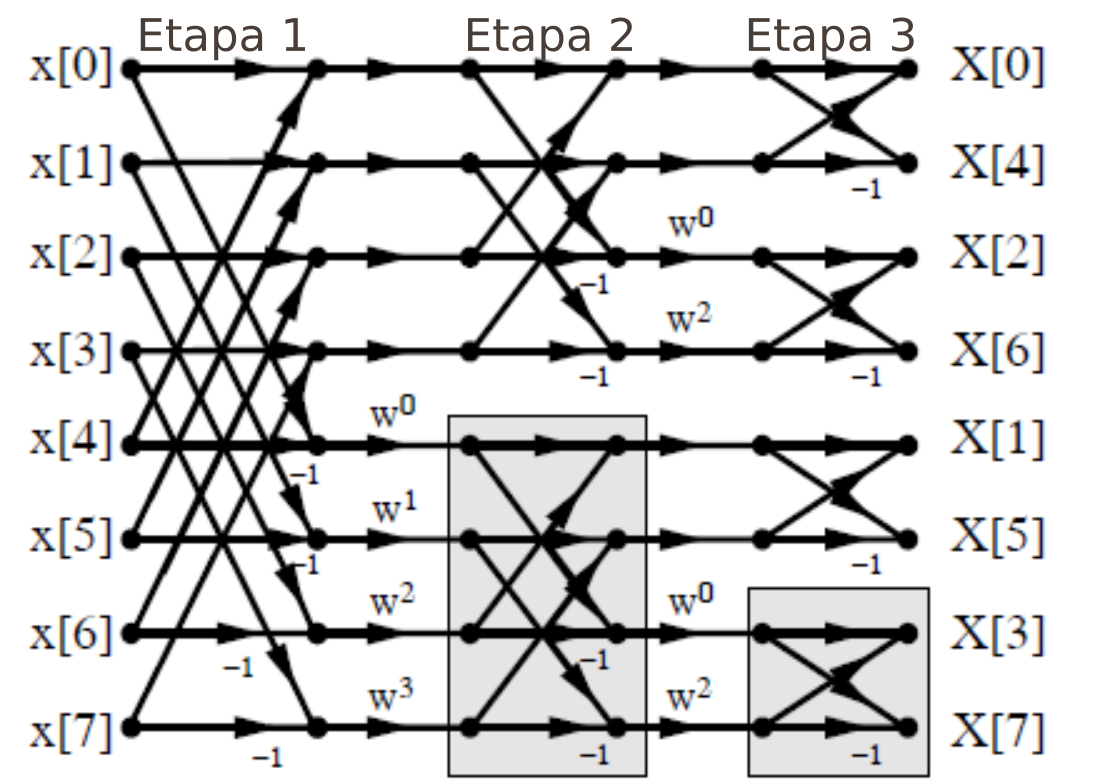
\includegraphics[scale=0.42]{./figures/r2_8.png}
%     \end{center}
%   \end{block}
%   
%   %\only<2-3>{
%   \begin{itemize}
%     \item<2-> Cada círculo representa una suma
%     \item<3-> Cada flecha representa un producto
%   \end{itemize}
  %}
%\end{frame}}
  
%   \only<4-5>{
%   \begin{itemize}
%     \item<4-> Existen varias alternativas de implementación de este algoritmo
%     \item<5-> Se diferencian en la forma en que se procesan las etapas del esquema
%   \end{itemize}}
%\end{frame}

\begin{frame}{Arquitecturas para la implementaci�n radix-r}
  \begin{itemize}
    \item<1-> Arquitectura paralela
    \uncover<2-5>{
      \begin{center}
	    \advance\leftskip-0.2cm
	    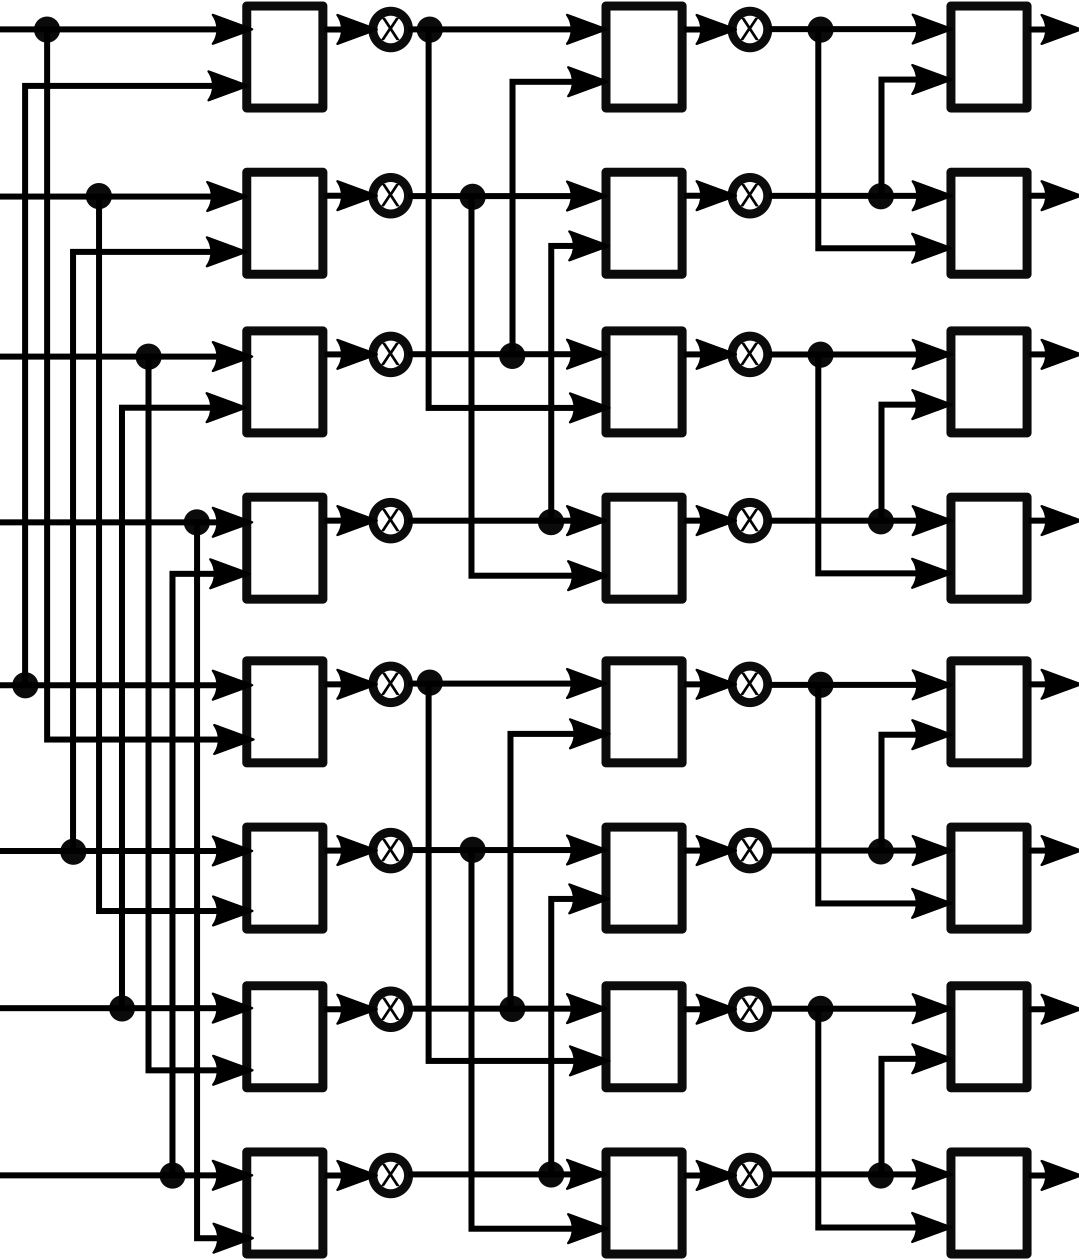
\includegraphics[scale=0.155]{./figures/r2_paralel.png}
      \end{center}
    }
    \item<1-> Arquitectura desenrrollada
    \uncover<3-5>{
      \begin{center}
	    \advance\leftskip-0.2cm
	    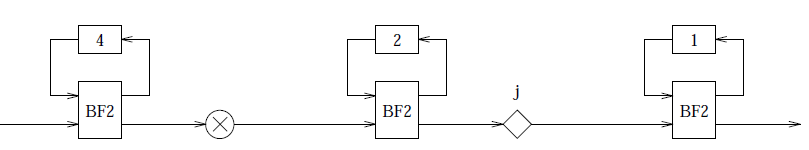
\includegraphics[scale=0.275]{./figures/r2sdf_8.png}
      \end{center}
%     \begin{itemize}
%       \item<8-> Un butterfly y un multiplicador por cada etapa
%       \item<9-> Bus serie
%       \item<10-> Pipeline
%     \end{itemize}
     }
    \item<1-> Arquitectura iterativa
    \uncover<4-5>{
      \alt<4>{
      \begin{center}
	    \advance\leftskip-0.2cm
	    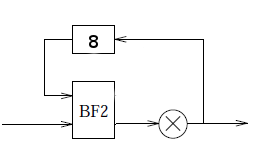
\includegraphics[scale=0.375]{./figures/r2sBf.png}
      \end{center}
      }{
      \begin{center}
	    \advance\leftskip-0.2cm
	    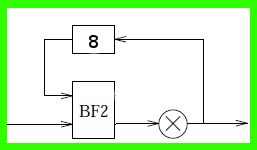
\includegraphics[scale=0.375]{./figures/r2sBf_sel2.png}
      \end{center}
      }
%     \begin{itemize}
%       \item<13-> Un único buterfly y un único multiplicador para todas las etapas
%     \end{itemize}
     }
  \end{itemize}
\end{frame}

% \begin{frame}{Selección de arquitectura radix}
%   \begin{center}
%     \advance\leftskip-0.2cm
%     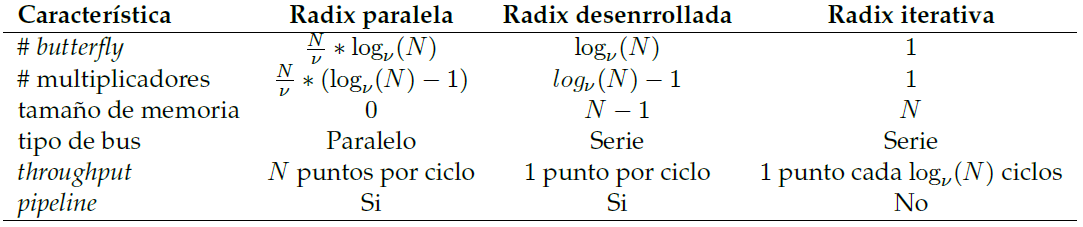
\includegraphics[scale=0.27]{./figures/radix_table.png}
%   \end{center}
%   
%   \begin{itemize}
%     \item<2-> Dado el requerimiento de la economía espacial y de recursos
% %     \item<3-> Y dado que el trhoughput no es fundamental
%     \item<3-> Se selecciona la arquitectura iterativa para la implementación de las arquitecturas
%     radix-2 y radix-4.
%   \end{itemize}
% \end{frame}
